\chapter{Continuous Expression Targets in \emph{EvoTSC}}
\label{chap:continuous}

In this chapter, I present the last line of work that I pursued during my PhD.

\section{A Continuous Target for Gene Expression}

\begin{figure}
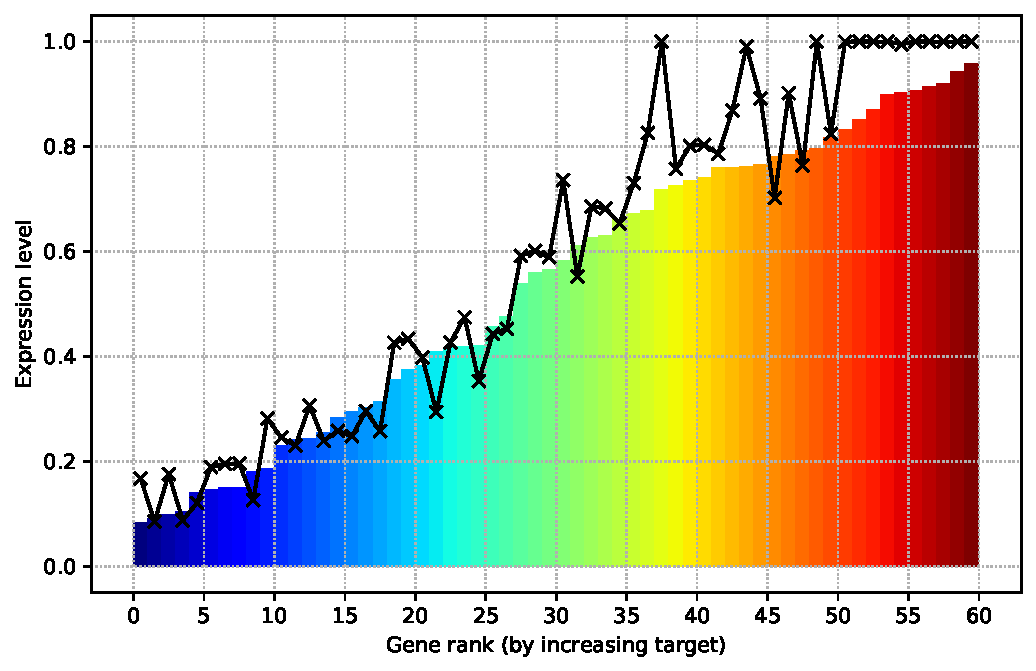
\includegraphics[width=0.495\textwidth]{continuous/img/best_rep00.pdf}
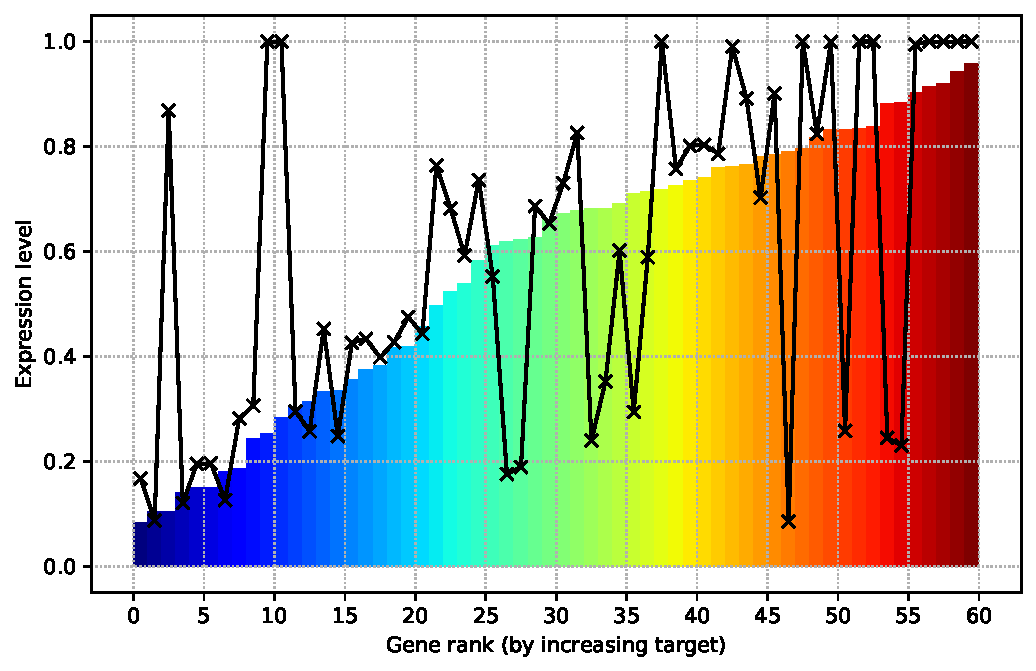
\includegraphics[width=0.495\textwidth]{continuous/img/shuffled.pdf}
\caption{Representation of an evolved and shuffled individual.}
\label{fig:continuous:indiv}
\end{figure}

\section{Results}

\subsection{Evolution of the Wild-Types}

\begin{figure}
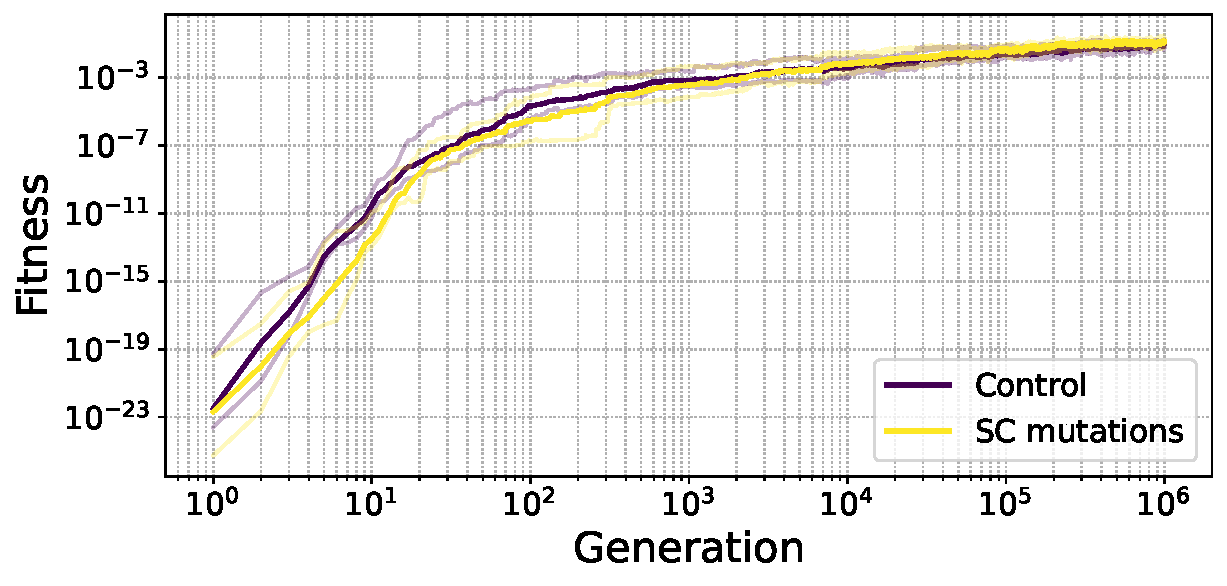
\includegraphics[width=\textwidth]{continuous/img/fitness_all_with_main.pdf}
\caption{Average fitness of the wild-types.}
\label{fig:continuous:wt-fitness}
\end{figure}

\begin{figure}
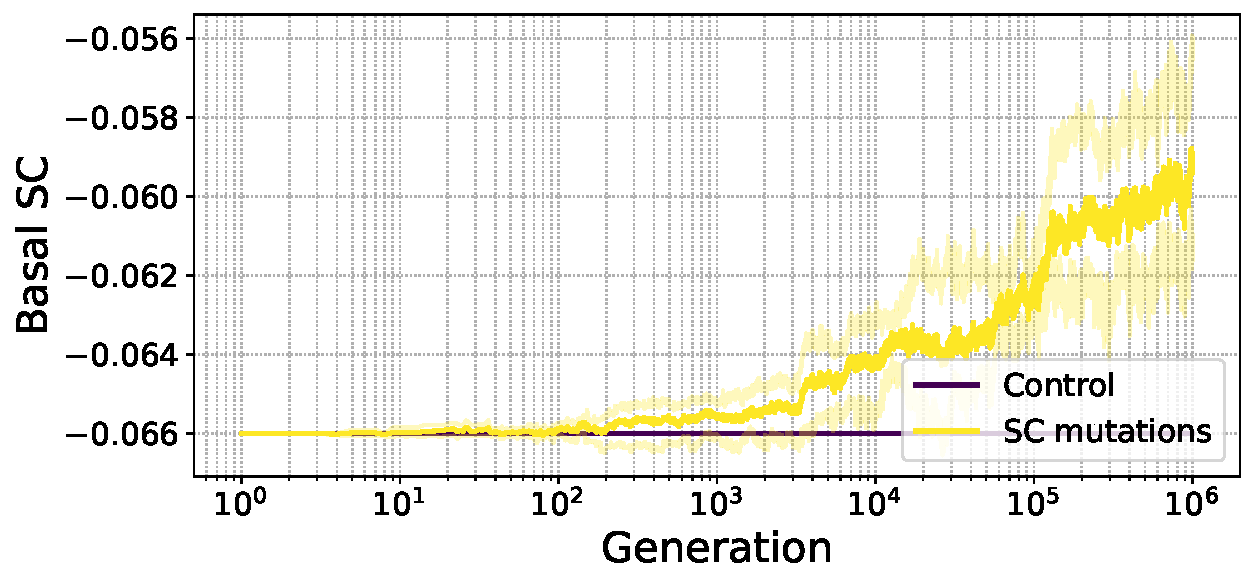
\includegraphics[width=\textwidth]{continuous/img/basal_sc_all.pdf}
\caption{Average supercoiling of the wild-types.}
\label{fig:continuous:wt-sc}
\end{figure}

\subsection{No Epistasis Found}

\begin{figure}
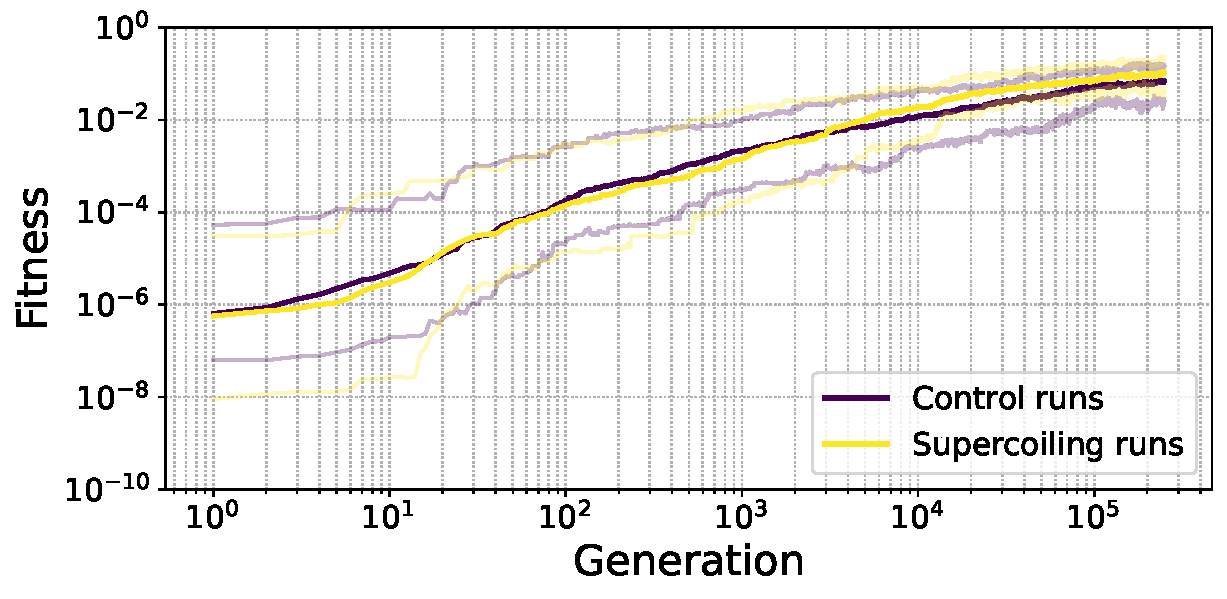
\includegraphics[width=\textwidth]{continuous/img/fitness_grouped.pdf}
\caption{Average fitness of the restarts.}
\label{fig:continuous:restart-fitness}
\end{figure}

\begin{figure}
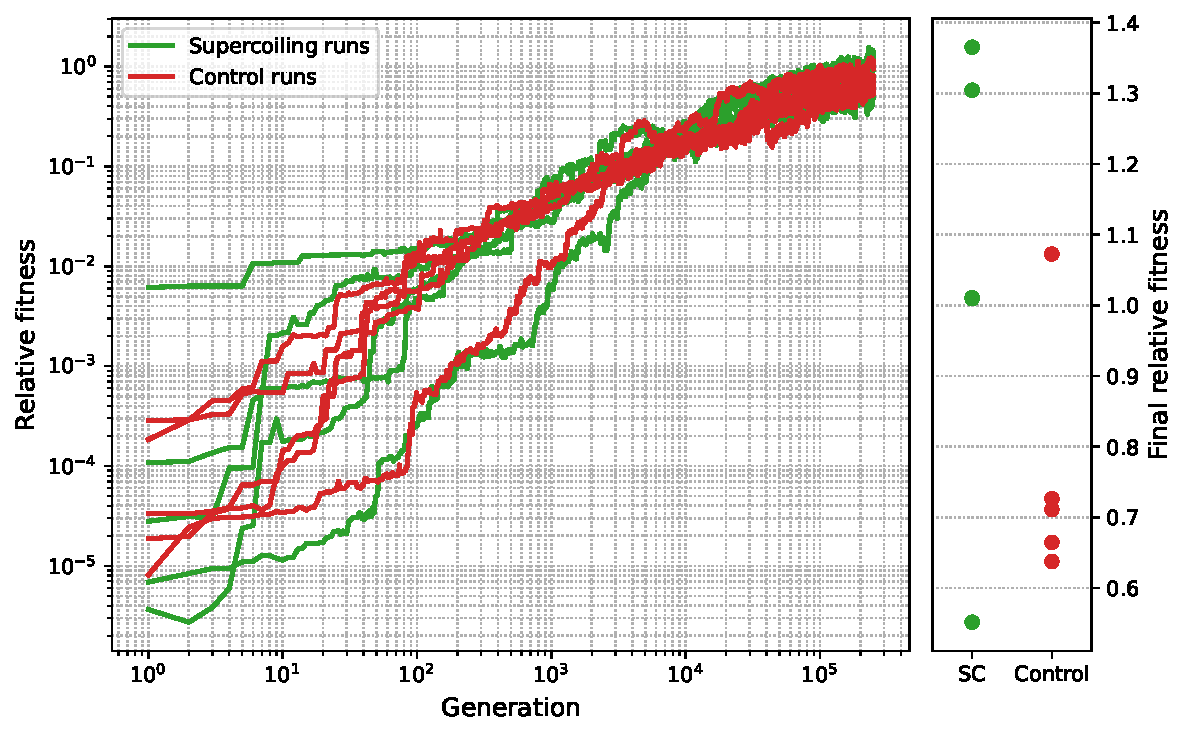
\includegraphics[width=\textwidth]{continuous/img/rel_fitness_sc_control.pdf}
\caption{Relative fitness of the restarts.}
\label{fig:continuous:restart-rel-fitness}
\end{figure}


\section{Discussion}

